\documentclass[12pt, a4paper]{article}
\usepackage[margin=0.5in]{geometry} 
\usepackage{tikz}


\title{\underline{8IM200}}
\date{} 
\begin{document} 
\maketitle 
\small {\underline{ F.M. 20} \hfill \underline{time : 20 min} } 
\vspace{5mm} 

\begin{enumerate}
\large

\item	Find the area of the following figure: 
\begin{center}
\tikzset{every picture/.style={line width=0.75pt}} %set default line width to 0.75pt        

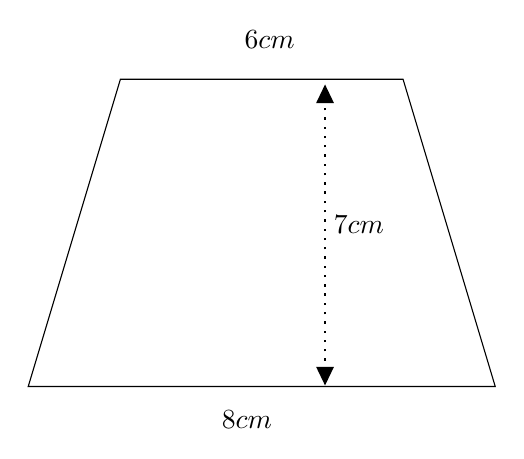
\begin{tikzpicture}[x=0.75pt,y=0.75pt,yscale=-1,xscale=1]
%uncomment if require: \path (0,300); %set diagram left start at 0, and has height of 300

\draw   (217,229) -- (261.4,81) -- (397.6,81) -- (442,229) -- cycle ;
%Straight Lines [id:da9150489185525186] 
\draw  [dash pattern={on 0.84pt off 2.51pt}]  (360,225.5) -- (360,86.5) ;
\draw [shift={(360,83.5)}, rotate = 450] [fill={rgb, 255:red, 0; green, 0; blue, 0 }  ][line width=0.08]  [draw opacity=0] (8.93,-4.29) -- (0,0) -- (8.93,4.29) -- cycle    ;
\draw [shift={(360,228.5)}, rotate = 270] [fill={rgb, 255:red, 0; green, 0; blue, 0 }  ][line width=0.08]  [draw opacity=0] (8.93,-4.29) -- (0,0) -- (8.93,4.29) -- cycle    ;

% Text Node
\draw (320,56.4) node [anchor=north west][inner sep=0.75pt]    {$6cm$};
% Text Node
\draw (309,239.4) node [anchor=north west][inner sep=0.75pt]    {$8cm$};
% Text Node
\draw (363,145.4) node [anchor=north west][inner sep=0.75pt]    {$7cm$};

\end{tikzpicture}
\end{center}
\item	Find the simple interest on Rs. 20000 at the rate of 4\% for 9 years. 

\item Find the amount after 3 years if you invest Rs. 62500 at the rate of 20\% compounded anually. 

\item
The cost of a pair of shoes is Rs.830. The sales tax charged on the shoes is 8\%. Find the bill amount. 

\item Find the perimeter of the following circle. 

\tikzset{every picture/.style={line width=0.75pt}}
\begin{center}
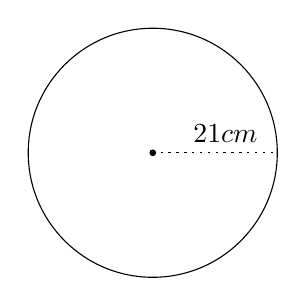
\begin{tikzpicture}[x=0.75pt,y=0.75pt,yscale=-1,xscale=1]
\draw (40,150) circle (60);
\filldraw (40,150) circle (1pt);
\draw [dash pattern={on 0.84pt off 2pt}] (40,150) -- (100,150); \draw (75,150) node[anchor=south]{$21cm$};
\end{tikzpicture}
\end{center}


\item Find $x$ in the following figure
\begin{center}
\tikzset{every picture/.style={line width=0.75pt}} %set default line width to 0.75pt        

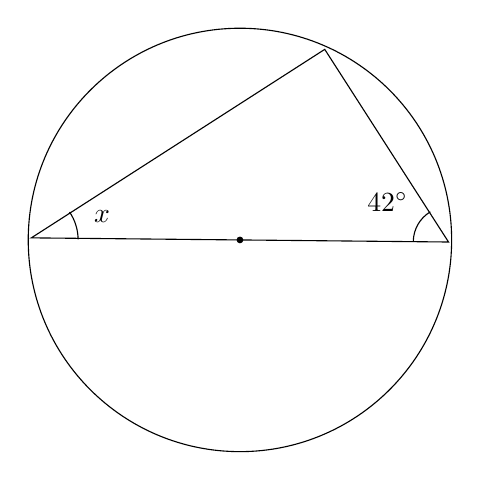
\begin{tikzpicture}[x=0.75pt,y=0.75pt,yscale=-1,xscale=1]
%uncomment if require: \path (0,300); %set diagram left start at 0, and has height of 300

%Shape: Circle [id:dp42205036788503136] 
\draw   (155,152.5) .. controls (155,96.17) and (200.67,50.5) .. (257,50.5) .. controls (313.33,50.5) and (359,96.17) .. (359,152.5) .. controls (359,208.83) and (313.33,254.5) .. (257,254.5) .. controls (200.67,254.5) and (155,208.83) .. (155,152.5) -- cycle ;

\filldraw (257,152.5) circle (1pt);
%Shape: Right Triangle [id:dp42281702403933297] 
\draw   (357.5,153.5) -- (156.5,151.5) -- (297.86,60.68) -- cycle ;
%Shape: Arc [id:dp5914382132660061] 
\draw  [draw opacity=0] (174.92,139.06) .. controls (177.63,143.07) and (178.97,147.64) .. (179.03,152.19) -- (155,152.5) -- cycle ; \draw   (174.92,139.06) .. controls (177.63,143.07) and (178.97,147.64) .. (179.03,152.19) ;
%Shape: Arc [id:dp21618776566863684] 
\draw  [draw opacity=0] (340.51,153.25) .. controls (340.59,147.21) and (343.85,141.88) .. (348.73,138.94) -- (357.5,153.5) -- cycle ; \draw   (340.51,153.25) .. controls (340.59,147.21) and (343.85,141.88) .. (348.73,138.94) ;

% Text Node
\draw (320.8,132) node [anchor=north west][inner sep=-2pt]    {$42^{\circ} $};
% Text Node
\draw (181.2,133) node [anchor=north west][inner sep=4pt]    {$x$};


\end{tikzpicture}
\end{center}

\item What is the volume of a cube of side $7cm$.

\item Find the height of the cuboid in the following figure if its  volume is $81cm^3$

\begin{center}
\tikzset{every picture/.style={line width=0.75pt}} %set default line width to 0.75pt        

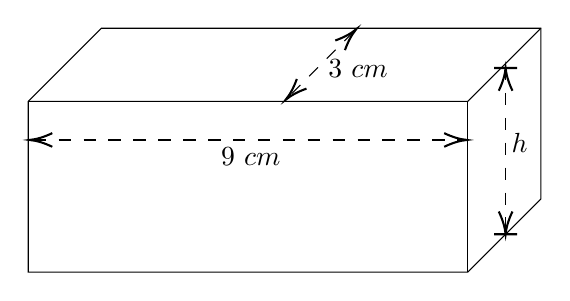
\begin{tikzpicture}[x=0.75pt,y=0.75pt,yscale=-1,xscale=1]
%uncomment if require: \path (0,300); %set diagram left start at 0, and has height of 300

%Shape: Cube [id:dp9473948708460411] 
\draw   (121,160.25) -- (156.25,125) -- (368,125) -- (368,207.25) -- (332.75,242.5) -- (121,242.5) -- cycle ; \draw   (368,125) -- (332.75,160.25) -- (121,160.25) ; \draw   (332.75,160.25) -- (332.75,242.5) ;
%Straight Lines [id:da9890251139395412] 
\draw  [dash pattern={on 4.5pt off 4.5pt}]  (277.59,126.91) -- (246.41,158.09) ;
\draw [shift={(245,159.5)}, rotate = 315] [color={rgb, 255:red, 0; green, 0; blue, 0 }  ][line width=0.75]    (10.93,-3.29) .. controls (6.95,-1.4) and (3.31,-0.3) .. (0,0) .. controls (3.31,0.3) and (6.95,1.4) .. (10.93,3.29)   ;
\draw [shift={(279,125.5)}, rotate = 135] [color={rgb, 255:red, 0; green, 0; blue, 0 }  ][line width=0.75]    (10.93,-3.29) .. controls (6.95,-1.4) and (3.31,-0.3) .. (0,0) .. controls (3.31,0.3) and (6.95,1.4) .. (10.93,3.29)   ;
%Straight Lines [id:da24744168549288137] 
\draw  [dash pattern={on 4.5pt off 4.5pt}]  (123.67,178.83) -- (330.33,178.83) ;
\draw [shift={(332.33,178.83)}, rotate = 180] [color={rgb, 255:red, 0; green, 0; blue, 0 }  ][line width=0.75]    (10.93,-3.29) .. controls (6.95,-1.4) and (3.31,-0.3) .. (0,0) .. controls (3.31,0.3) and (6.95,1.4) .. (10.93,3.29)   ;
\draw [shift={(121.67,178.83)}, rotate = 0] [color={rgb, 255:red, 0; green, 0; blue, 0 }  ][line width=0.75]    (10.93,-3.29) .. controls (6.95,-1.4) and (3.31,-0.3) .. (0,0) .. controls (3.31,0.3) and (6.95,1.4) .. (10.93,3.29)   ;
%Straight Lines [id:da9647081910606832] 
\draw  [dash pattern={on 4.5pt off 4.5pt}]  (351,144.17) -- (351,224.25) ;
\draw [shift={(351,224.25)}, rotate = 270] [color={rgb, 255:red, 0; green, 0; blue, 0 }  ][line width=0.75]    (0,5.59) -- (0,-5.59)(10.93,-3.29) .. controls (6.95,-1.4) and (3.31,-0.3) .. (0,0) .. controls (3.31,0.3) and (6.95,1.4) .. (10.93,3.29)   ;
\draw [shift={(351,144.17)}, rotate = 90] [color={rgb, 255:red, 0; green, 0; blue, 0 }  ][line width=0.75]    (0,5.59) -- (0,-5.59)(10.93,-3.29) .. controls (6.95,-1.4) and (3.31,-0.3) .. (0,0) .. controls (3.31,0.3) and (6.95,1.4) .. (10.93,3.29)   ;

% Text Node
\draw (264.33,138.9) node [anchor=north west][inner sep=0.75pt]    {$3\ cm$};
% Text Node
\draw (212.67,181.07) node [anchor=north west][inner sep=0.75pt]    {$9\ cm$};
% Text Node
\draw (352.67,174.57) node [anchor=north west][inner sep=0.75pt]    {$h$};


\end{tikzpicture}

\end{center}

\item
Find the area of a circle if its perimeter is $44cm$.

\item Find the volume of the following figure
\begin{center}
\tikzset{every picture/.style={line width=0.75pt}} %set default line width to 0.75pt        

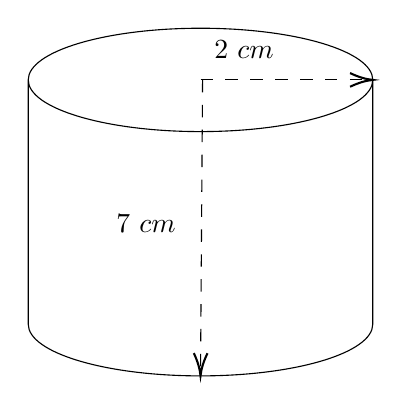
\begin{tikzpicture}[x=0.75pt,y=0.75pt,yscale=-1,xscale=1]
%uncomment if require: \path (0,300); %set diagram left start at 0, and has height of 300

%Shape: Can [id:dp3005694542431201] 
\draw   (366,84.9) -- (366,202.6) .. controls (366,216.35) and (328.84,227.5) .. (283,227.5) .. controls (237.16,227.5) and (200,216.35) .. (200,202.6) -- (200,84.9) .. controls (200,71.15) and (237.16,60) .. (283,60) .. controls (328.84,60) and (366,71.15) .. (366,84.9) .. controls (366,98.65) and (328.84,109.8) .. (283,109.8) .. controls (237.16,109.8) and (200,98.65) .. (200,84.9) ;
%Straight Lines [id:da14639871862648146] 
\draw  [dash pattern={on 4.5pt off 4.5pt}]  (283,84.9) -- (364,84.9) ;
\draw [shift={(366,84.9)}, rotate = 180] [color={rgb, 255:red, 0; green, 0; blue, 0 }  ][line width=0.75]    (10.93,-3.29) .. controls (6.95,-1.4) and (3.31,-0.3) .. (0,0) .. controls (3.31,0.3) and (6.95,1.4) .. (10.93,3.29)   ;
%Straight Lines [id:da7426914554244644] 
\draw  [dash pattern={on 4.5pt off 4.5pt}]  (284,84.9) -- (283.01,225.5) ;
\draw [shift={(283,227.5)}, rotate = 270.4] [color={rgb, 255:red, 0; green, 0; blue, 0 }  ][line width=0.75]    (10.93,-3.29) .. controls (6.95,-1.4) and (3.31,-0.3) .. (0,0) .. controls (3.31,0.3) and (6.95,1.4) .. (10.93,3.29)   ;

% Text Node
\draw (288.4,64.8) node [anchor=north west][inner sep=0.75pt]    {$2\ cm$};
% Text Node
\draw (241.2,148.6) node [anchor=north west][inner sep=0.75pt]    {$7\ cm$};


\end{tikzpicture}
\end{center}

\end{enumerate}

\end{document}


